\documentclass[12pt,a4paper]{report}
% Packages for enhanced functionality
\usepackage[utf8]{inputenc}
\usepackage[T1]{fontenc}
\usepackage{graphicx} % For including images
\usepackage{geometry} % For page layout
\usepackage{hyperref} % For clickable links and references
\usepackage{fancyhdr} % For custom headers and footers
\usepackage{titlesec} % For section title formatting
\usepackage{float} \usepackage{circuitikz}
\usepackage{caption}
\usepackage{siunitx}
\usepackage{amsmath}
\usepackage{tikz}
\usepackage{subcaption}
\usepackage{booktabs}
\newcommand{\vecb}[1]{\mathbf{#1}}
\newcommand{\brak}[1]{\ensuremath{\left(#1\right)}}
\newcommand{\cbrak}[1]{\ensuremath{\left\{#1\right\}}}
\newcommand{\abs}[1]{\left\vert#1\right\vert}
\newcommand{\norm}[1]{\left\lVert#1\right\rVert}
\providecommand{\sbrak}[1]{\ensuremath{{}\left[#1\right]}}
\providecommand{\lsbrak}[1]{\ensuremath{{}\left[#1\right.}}
\providecommand{\rsbrak}[1]{\ensuremath{{}\left.#1\right]}}
\providecommand{\brak}[1]{\ensuremath{\left(#1\right)}}
\providecommand{\lbrak}[1]{\ensuremath{\left(#1\right.}}
\providecommand{\rbrak}[1]{\ensuremath{\left.#1\right)}}
\providecommand{\cbrak}[1]{\ensuremath{\left\{#1\right\}}}
\providecommand{\lcbrak}[1]{\ensuremath{\left\{#1\right.}}
\providecommand{\rcbrak}[1]{\ensuremath{\left.#1\right\}}}
\hypersetup{
    colorlinks=true,  % Enable colored text links
    linkcolor=orange,    % Internal links (sections, table of contents, etc.)
    urlcolor=orange,     % External URLs
    citecolor=orange,    % Citations
    pdfborder={0 0 0} % Remove ugly default borders
}
\begin{document}
\title{\textbf{Experiment 5}\\
\LARGE{\textbf{ }}
\author{Akshara Sarma (EE224BTECH11003 \\ Arjun Pavanje (EE24BTECH11005)}

\begin{center}
\end{center}
\vspace{30pt}
\begin{figure}[ht]
	\centering
	
\includegraphics[width = 100pt]{logo.png}\\
\end{figure}
\begin{center}
	Bachelor of Technology\\
	\vspace{10pt}
	Department of Electrical Engineering\\
\end{center}
}
\maketitle
\section{Aim}
\begin{enumerate}
\item Measure the DC I–V characteristic of a diode and extract diode parameters (ideality factor $\mathbf{n}$ and saturation current $\mathbf{I_s}$). 
\item Measure the small-signal (dynamic) resistance $\mathbf{r_d}$ around a chosen bias point and verify the small-signal model. 
\item Further, bias the diode with a DC voltage and apply a small AC signal. Observe the output on the CRO and use FFT mode to see harmonics. The diode current is nonlinear,
\begin{align*}
I \approx I_0 + g_1v + \frac{1}{2}g_2*v^2.
\end{align*}
\begin{itemize}
\item For small $V_{ac}$, only the fundamental appears. 
\item As $V_{ac}$ increases, 2nd and higher harmonics appear, showing nonlinearity. 
\item Measure fundamental and 2nd harmonic amplitudes vs $V_{ac}$ and note slopes $~1$ and $~2$
\end{itemize}
\end{enumerate}

\section{I-V characteristics of Diode}
$V_d$ (diode voltage) is calculated for multiple values of $V_s$ (source voltage).
\begin{figure}[!ht]
\centering
\resizebox{0.5\textwidth}{!}{%
\begin{circuitikz}
\tikzstyle{every node}=[font=\normalsize]
\draw (3.75,12.5) to[american voltage source,l={ \normalsize $V_s$}] (3.75,10);
\draw (3.75,12.5) to[R,l={ \normalsize R}] (6.25,12.5);
\draw (6.25,12.5) to[D,l={ \normalsize 1N4007}] (6.25,10);
\draw (6.25,10) to[short] (3.75,10);
\end{circuitikz}
}%
\end{figure}
\pagebreak
\begin{table}[h!]
\centering
\begin{tabular}{|c|c|}
\hline
$V_s$ (V) & $V_d$ (V) \\
\hline
0.0 & 0.0 \\
0.1 & 0.143 \\
0.2 & 0.250 \\
0.4 & 0.399 \\
0.6 & 0.478 \\
0.8 & 0.519 \\
1.0 & 0.544 \\
1.2 & 0.560 \\
1.4 & 0.571 \\
1.6 & 0.579 \\
1.8 & 0.588 \\
2.0 & 0.595 \\
2.2 & 0.601 \\
2.4 & 0.608 \\
2.6 & 0.614 \\
2.8 & 0.617 \\
3.0 & 0.621 \\
3.2 & 0.626 \\
3.4 & 0.629 \\
3.6 & 0.633 \\
3.8 & 0.636 \\
4.0 & 0.639 \\
4.2 & 0.641 \\
4.4 & 0.644 \\
4.6 & 0.647 \\
4.8 & 0.649 \\
5.0 & 0.652 \\
\hline
\end{tabular}
\end{table}
\newline We require the exponential curve that is closest to all the obtained data points. So curve-fitting must be done. Scipy's curve$\_$fit was used. $I_s, \eta$ was calculated using the same python code.
\pagebreak
\begin{figure}[h!]
    \centering
    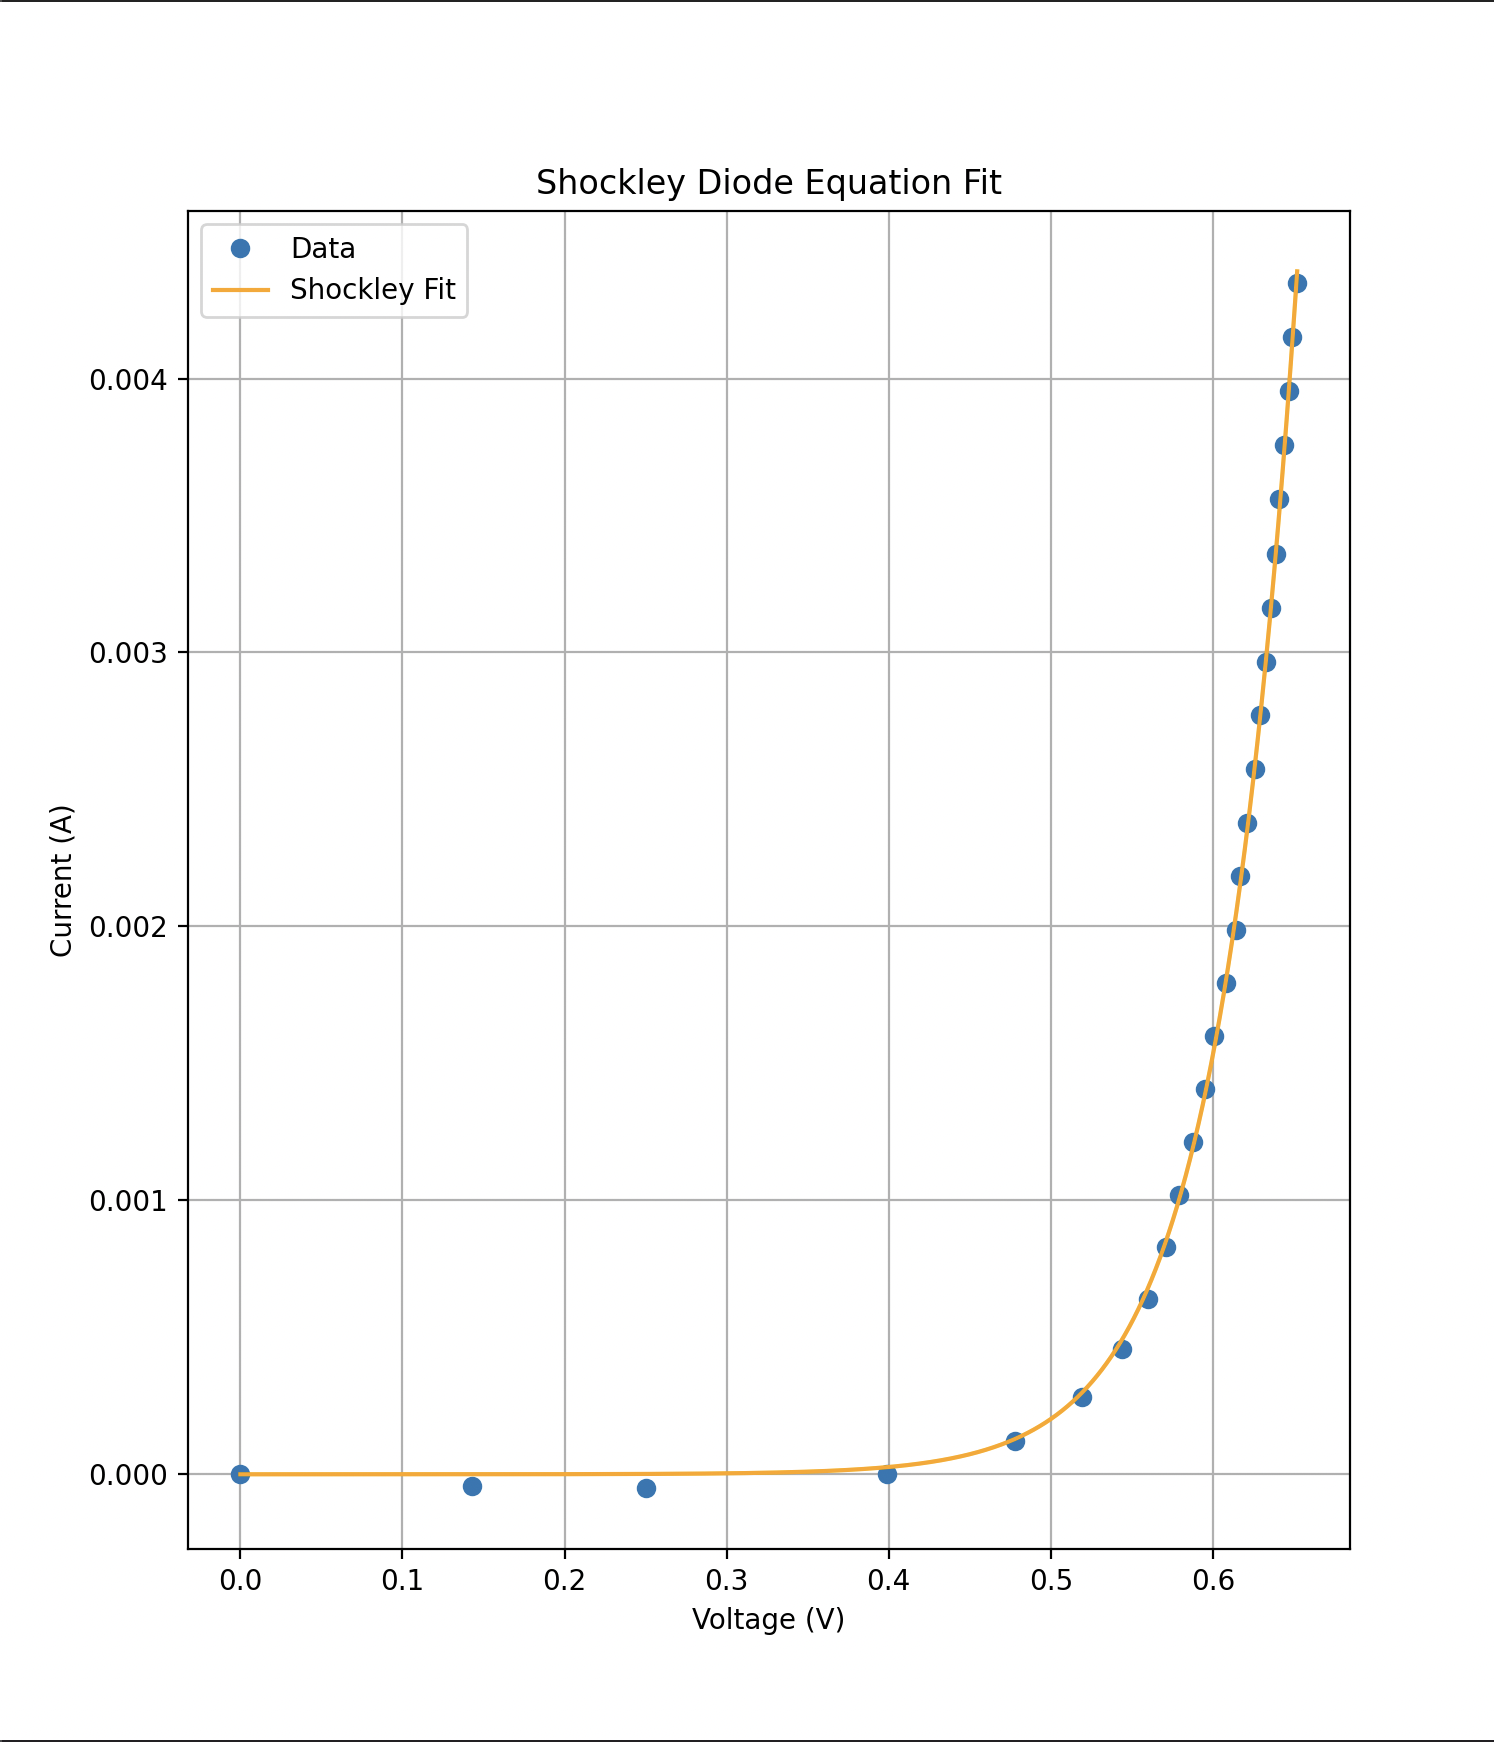
\includegraphics[width=0.7\linewidth]{figs/curve_fit.png}
\end{figure}
\newline We obtain diode parameters,
\begin{itemize}
    \item Ideality factor ($\eta$) = $1.907$
    \item Saturation current ($I_s$) = $8.109nA$
\end{itemize}
\pagebreak
\section{Small Signal Analysis}
After fixing a bias point, a sine-wave of very small amplitude was applied to calculate small signal characteristics.
\begin{figure}[!ht]
\centering
\resizebox{0.6\textwidth}{!}{%
\begin{circuitikz}
\tikzstyle{every node}=[font=\normalsize]
\draw (3.75,12.5) to[american voltage source,l={ \normalsize $V_s$}] (3.75,10);
\draw (3.75,12.5) to[R,l={ \normalsize R}] (6.25,12.5);
\draw (6.25,12.5) to[D,l={ \normalsize 1N4007}] (6.25,10);
\draw (3.75,10) to[sinusoidal voltage source, sources/symbol/rotate=auto,l={ \normalsize $V_{ac}$}] (6.25,10);
\end{circuitikz}
}%
\end{figure}
\newline We pick 2 points and note $V_S, V_D$ values.
\begin{table}[h!]
\centering
\begin{tabular}{|c|c|}
\hline
$V_s$ & $V_d$ \\
\hline
3.960 & 3.018 \\
2.040 & 2.982 \\
\hline
\end{tabular}
\end{table}
\newline Small signal parameter $r_d$ is calculated (for bias point $V_D = 3V$) as,
\begin{itemize}
    \item Theoretical: $\frac{\eta V_T}{I_D} = 20.69782927852349\Omega$
    \item Calculated: $\frac{\Delta V_D}{\Delta I_D} = 19.108280254776847\Omega$
\end{itemize}
$I_D$ is found by $\frac{V_S - V_D}{R}$. $\eta$ value calculated previously is used in theoretical calculation.
\pagebreak
\section{FFT Harmonics}
To observe FFT harmonics we reuse the circuit built previously,
\begin{figure}[!ht]
\centering
\resizebox{0.6\textwidth}{!}{%
\begin{circuitikz}
\tikzstyle{every node}=[font=\normalsize]
\draw (3.75,12.5) to[american voltage source,l={ \normalsize $V_s$}] (3.75,10);
\draw (3.75,12.5) to[R,l={ \normalsize R}] (6.25,12.5);
\draw (6.25,12.5) to[D,l={ \normalsize 1N4007}] (6.25,10);
\draw (3.75,10) to[sinusoidal voltage source, sources/symbol/rotate=auto,l={ \normalsize $V_{ac}$}] (6.25,10);
\end{circuitikz}
}%
\end{figure}
\newline To observe harmonics of $I_D$ we can just observe resistor voltage ($V_S-V_D$) as it is just a scaled version ($RI_D$) of diode current. When $V_{ac}$ is very small, we observe only one peak at frequency $f$ (frequency of sinusoidal signal). As we increase $V_{ac}$, number of peaks increases and the peaks occur at $f, 2f, 3f, \cdots$.
\end{document}